\documentclass{article}
\usepackage[utf8]{inputenc}
\usepackage{graphicx}
\graphicspath{ {./images/} }
\usepackage{booktabs}
\usepackage{hyperref}
\usepackage{xcolor}
\usepackage{setspace}
\usepackage{indentfirst}
\usepackage{float}
\usepackage{hanging}
\usepackage[bottom]{footmisc}
\setlength{\parskip}{5pt}


\title{% 
  Tax Revenue Cyclicality and Income Inequality: \\
  Evidence from U.S. Counties From 1989 to 2019 \\
  \vspace{5mm}
  }

\author{
    Yiyang Chen\footnote{\normalsize{(Email: yiyangc@berkeley.edu) I would like to thank Professor Emi Nakamura for advising this senior thesis and offering very helpful comments and suggestions. This work is not possible without her help.} } 
    \vspace{5mm}
    \\
    Deparment of Economics \\
    University of California, Berkeley
}

\date{May 2022}

\begin{document}

\maketitle

\pagebreak

% ############
% ABSTRACT
% ############

\begin{center}
\textbf{Abstract}
\end{center}

Tax revenue is known to be pro-cyclical--it increases when the economy is booming, and falls when a recession takes over. It is important to understand the exact dynamics of these cyclical fluctuations of tax revenue as many offerings of the public goods, on top of other things, depend on the government budget, especially on a local level. Therefore, it is worthwhile to consider various factors that may have either strengthened or lessened the impact of business cycles on government tax revenue. 

In my paper, I will examine how income inequality may be associated with the cyclicality of tax revenue chiefly using U.S. county individual taxable income data from 1989-2019. I will perform a panel regression analysis looking at how tax revenue cyclicality in each county varies by income inequality at the respective location. I find that the effect is significant across counties in the same time period, where counties with higher inequality tend to have a more volatile cyclical fluctuation of local tax revenue. However, it seems the rising income inequality over the past few decades had relatively small impact on tax revenue being more sensitive to the business cycle. 

\begin{flushleft}
\textbf{Keywords:} tax revenue, individual income tax, tax volatility, business cycles, income inequality
\end{flushleft}

\pagebreak

% ############
% INTRODUCTION 
% ############


\section{Introduction}

A desirable characteristic of government tax revenue is its pro-cyclicality, i.e. when the economy is good, the tax revenue is higher; when the economy is in the midst of a crisis, the tax revenue is lower. This automatic adjustment helps, to some extent, keeping the economy at equilibrium. However, the cyclical fluctuations are also creating problems for policymakers as it is important to understand the exact dynamics of these cyclical fluctuations of tax revenue as many offerings of the public goods, on top of other things, depend on the government budget, especially on a local level. Changes in local tax revenue influence local government's capacity of, for example, funding education, highways and social programs such as Medicaid that rely on stable state and local finances. 

These public investments in education, infrastructure, and social services are not only crucial to local citizens but can also contribute to the overall economic growth. Yet they are running at risk if a strong and consistent flow of tax revenue cannot be secured. For instance, the high degree of fiscal stress experienced by state governments in the 2001 and the 2007–2009 recessions has demonstrated governments did not fully understand the tax revenue dynamics, and thus were not very well prepared. On top of that, recessions are not rare economic events; instead they are part of the economic cycle, as aggregate demand in the economy expands and contracts over time and recessions occur during prolonged contractions. 

So being able to make good predictions of tax revenue based on the business cycle can help local authorities better manage their finances and budget. To do so, we must understand what can lead to varying sensitivity of which tax revenue responds to business cycle--in some places, a small business cycle movement can lead to a huge change in tax revenue, and in other places, not so much. Therefore, it is worthwhile to consider various factors that may have either strengthened or lessened the impact of the business cycle on government tax revenue. 

This paper will mainly consider how local income inequality may contribute to individual income tax revenue. The logic behind this link is straightforward. In places with high income inequality, we tend to see a higher portion of personal income coming from the top income population. Income volatility tends to be greater among higher-income groups because households in such groups derive a large portion of their income from capital income rather than relatively more stable wages and salaries. Since capital income fluctuates more in response to economic conditions than labor income does, when those fluctuations ultimately affect the income of individual households, they will lead to more volatile movements of local individual income tax revenue. 

So the first question the paper will attempt to answer is whether empirical data support the premise I made above: higher income inequality can give rise to more volatile cyclical fluctuations of tax revenue. Another natural follow-up question is how the growing income inequality for the past few decades has changed its dynamics. According to statistics compiled by the Congressional Budget Office (CBO), households in the highest income quintile, which received about 55 percent of all income, paid more than two-thirds of all federal taxes in 2018. In contrast, the figure was 33 percent in 1993. Inequality economists describe ``the U.S. economy has been characterized by high economic inequality and a lack of strong, stable, and broadly shared economic gains and well-being. Economic power at the top has translated into social and political power coalesced among an elite few. Those who start with economic advantages are able to design a system of economic inequality that preserves and amplifies their position at the top, to the detriment of the rest of us and the public good." (Boushey 2019) So the result of this paper may also offer insights on how high income inequality can have a destabilizing effect on state and local finances, especially when the economy is in recessions. 

In my paper, I will examine how income inequality may be associated with the cyclicality of tax revenue chiefly using U.S. county individual taxable income data from 1989-2019. I will perform a panel regression analysis looking at how tax revenue cyclicality in each county varies by income inequality at the respective location. These results may help policymakers to understand and hopefully mitigate the sensitivity of tax revenues to economic conditions in order to secure steady state and local finances. 






% ##########
% LIT REVIEW
% ##########

\vspace{2mm}
\section{Literature Review}

Literature in tax revenue and income inequality provides a theoretical foundation for my premise to be valid. I will discuss in this section the way tax revenue is connected to the business cycle and possible reasons behind a more sensitive response given higher income inequality. 

One of the previous examinations of the cyclical behavior of aggregate and local tax revenue was done by Kodrzycki. In her paper ``Smoothing State Tax Revenues over the Business Cycle: Gauging Fiscal Needs and Opportunities", Kodrzycki used coincident index to indicate the variations in economic activities, and found a significant correlation between tax revenue and the coincident index both in aggregate level and on state level. A comparison was also made to explore the difference of tax elasticities between in 1980s, 1990s and in 2000s, and she found that most states experienced greater cyclical sensitivity in the 2000s than in the 1980s and 1990s, and ``the greater cyclical volatility of tax receipts in the 2000s can be traced to the fluctuations in personal income tax receipts. The elasticity of total tax revenue with respect to personal income was 0.83 in the 1980s to 1990s, and then increased to 1.76 in the 2000s." Kodrzycki also conducted a cross-section regressions, and it revealed that the main source of variation in income tax elasticities across states during the 2000s was the cyclical sensitivity of their residents' incomes as reflected on their federal income tax
returns. By contrast, she found that state-specific features such as the tax treatment of capital gains or the progressivity of tax rates did not account for significant differences in revenue elasticities across states. In addition, state departures from the federal definitions of adjusted gross income and taxable income, on the whole, did not contribute to increased revenue volatility over the business cycle. These findings are very important because they validate the assumption that differences in local tax treatment may not contribute substantially to our results. 

In addition, Kodrzycki also probed the cyclicality of tax revenue of different income sources. Kodrzycki estimated elasticity of wages and salaries to be unchanged from 1980s to early 2000s, which remained at around 0.8. One possible complication, she argued, was that this may be a result of the coincident index becoming less volatile in the 2000s relative to its prior history, while the personal income trend did not. However, when examining investment income, it became clear that volatility has risen in more recent years. ``During the 1980s and 1990s, a 1 percentage point increase in personal income was associated with a 1.13 percent increase in overall investment income and a 2.21 percent increase in capital gains. During the 2000s, these responses rose dramatically to 4.68 percent and 4.03 percent, respectively."

Kodrzycki's paper provides a solid background for my exploration of tax revenue cyclicality, and suggests many ways in which tax revenue can vary across time, geographical locations, and different income sources. It also offers insights into the reason behind the increased volatility, which I will examine in my paper. 

Other research also confirms this result. Sancak et al. examined tax revenue during the business cycle by estimating the relationship between tax revenue efficiency and the output gap using data from 1995 to 2008 for 32 EU countries, and also for 84 advanced and developing economies. Their analysis focused particularly on the value-added tax (VAT) C-efficiency. McGranahan and Mattoon at the Chicago Fed agreed that tax revenue has become more sensitive to changing economic conditions since the turn of the century. In addition to documenting increased volatility of tax revenue, they also attempted to explain the reason behind this movement. They made an enlightening comparison between investment income and S\&P 500 index, and observed that the major drops in investment income occurred along with major drops in stock market returns. Also, changes in capital gains tax policy as part of the Jobs and Growth Tax Relief Reconciliation Act of 2003 may have influenced investors' decisions concerning when to take gains and in which amount. McGranahan and Mattoon also offer suggestions for what state governments might do to better manage their tax revenues to avoid or minimize dramatic fiscal downturns, including adjusting tax-revenue-setting policy, and restructuring income tax to rely more on wages and salaries. 

As we now understand increased cyclicality of tax revenue can be a direct result from more volatile investment income, it is critical to see how this component will play out in the aggregate setting. The Congressional Budget Office provided a very valuable analysis of household income distribution from 1979 to 2018. They presented income growth trends for the groups of highest and lowest income households (see figure 2.1), and it showed clearly that income of the top income population is much more cyclical than the other. And their analysis confirms with the findings by McGranahan and Mattoon that ``income volatility tends to be greater among higher-income groups because households in such groups derive a large portion of their income from capital income, which fluctuates more in response to economic conditions than labor income does. Those fluctuations affect the income of individual households, contributing to the year-to-year changes in the set of households included in higher-income groups."

\begin{center}
Figure 2.1: Cumulative Growth in Income Before Transfers and Taxes Among Households in the Highest Quintile, 1979 to 2018\\
\noindent
\makebox[\textwidth]{
\includegraphics[scale=0.6]{images/literature/57061-ex04_income-before-growth-topq.png} }
\noindent Data source: Congressional Budget Office. The Distribution of Household Income, 2018. Aug 2021. https://www.cbo.gov/publication/57404. Accessed on 10 Apr. 2022
\end{center}

These previous works naturally lead to the discussion of income inequality, especially with the very top income group contributing heavily to the tax revenue volatility. It may be reasonable to consider if increased cyclicality of tax revenue will be an additional side effect of high income inequality. There are several papers that discuss this matter. Arnum et al. presented a historical overview of the late 20th-century advent of financialization, that is, the unprecedented growth of the financial sector. They summarized its origins and consequences, particularly greater income inequality, and concluded that along with higher unemployment and an eroding minimum wage, the growth of the U.S. financial sector had contributed to the exacerbation of inequality in recent decades. Owyang and Shell explored how financial crises affected high-income earners disproportionately because of their exposure to riskier assets. And they argued that the increase in income inequality in the 1970s was accompanied, in part, by gains in the stock market. Co-movement between stock prices and income inequality results from the fact that gains in the stock market tend to benefit those in the wealthiest portion of the income distribution, who have better access to and higher participation in these asset markets. 

In this paper, I will contribute to the existing literature by testing if and how cyclicality of tax revenue is associated with income inequality, with a particular focus on individual taxable income. This will provide empirical evidence to the underlying rationale discussed above. 






% ############
% DATA
% ############


\vspace{2mm}
\section{Data}

In this section, I will present the data and their sources used in my analysis, and describe the data manipulation methods applied to raw data. 

\subsection{County-Level Statistics}
\subsubsection{Income Tax}
U.S. county-level individual income data obtained from the Internal Revenue Service will be the main statistics used in my following analysis. Note that the tax statistics are not available before 2011, so here I will use the taxable income as an approximation. The relationship between tax revenue and total taxable income are reasonably stable, so changes in taxable income are highly likely to share similar trends with changes in tax revenue.

\begin{center}
Figure 3.1: Tax Revenue and AGI, 2011 to 2019\\
\noindent
\makebox[\textwidth]{
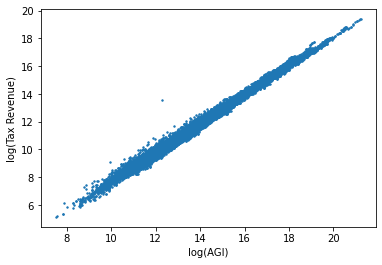
\includegraphics[scale=0.45]{images/data/tax_revenue_vs_agi.png} }
\noindent Note: The scatterplot uses data from 2011 to 2019 when both total tax liability and taxable income statistics are available. Tax revenue is given by the total tax liability. The figure demonstrates that the relationship between tax revenue and AGI is very stable during 2011-2019, it is reasonable to use changes in AGI as an approximation of changes in tax revenue.
\end{center}

However, using taxable income to approximate tax revenue admittedly involves a few limitations. First, it is unable to capture  the nonlinearity of tax revenue given taxable income as tax rates vary for different levels of earnings. Second, it fails to account for different tax rates given different sources of income (for example, capital gain has a different tax rate from salaries). Last, it may leave out many crucial impacts of changing tax policies over time. 

The IRS individual taxable income data consists of personal income data in 1,968 U.S. counties through 1989-2019. Before 2010, the annual datasets recorded the number of returns, the number of exemptions, the adjusted gross income (AGI), and personal income belonging to three income sources--wages and salaries, dividend income, interest income. The IRS data later than 2010 contains a more detailed breakdown of personal income of additional sources, including net capital gains, pensions and annuities, etc. These data of additional income sources would be extremely valuable if observations were available prior to 2010; however, in order to keep everything consistent, I will only take into account wages and salaries, dividend income, and interest income as the three income sources in my analysis. 

In addition, I will only keep counties which have annual percent changes in number of returns, number of exemptions, AGI, and income from different sources within the range of -50.0\% to 100.0\% during 1989-2019, and drop the remaining counties as outliers. Some outliers attribute to an IRS data error; some outliers (in particular, very large changes in dividend and interest income around 2010) may be the results of the Global Financial Crisis. See Appendix A for a discussion on the outliers.  

The county panel data ends up consisting of 1,941 counties, covering 64\% of all U.S. counties. Table 3.2 reports the summary statistics.
\begin{table}[H]\centering
\renewcommand\thetable{3.2}
\caption{Summary Statistics for County-Level Statistics}
\centerline{
    \begin{tabular}{lrrrr}
    \toprule
    \textbf{Variable} &  \textbf{Mean} &  \textbf{Standard} &  \textbf{Minimum} &   \textbf{Maximum} \\
    {} & {} & \textbf{deviation} & {} \\
    \midrule
    Gini Coefficient                &      0.43 &      0.04 &     0.31 &      0.65 \\
    Change in AGI                   &      4.21 &      6.17 &   -41.36 &     99.34 \\
    Change in Wages and Salaries    &      3.96 &      4.36 &   -42.37 &     91.39 \\
    Change in Dividend Income       &      5.26 &     17.45 &   -49.98 &     99.92 \\
    Change in Interest Income       &     -1.77 &     17.01 &   -49.96 &     98.34 \\
    \bottomrule
    \end{tabular}
}
\vspace{2mm}
Note: Changes are in percentages.
\end{table}


\subsubsection{Income Inequality}
County-level income inequality measures are aggregated from two sources. 

First, 1990 and 2000 Current Population Survey (CPS) conducted by Census Bureau provides income inequality data (Gini coefficients) for earlier periods. I will use 1990 Census estimates to approximate inequality measurements from 1989-1995, and 2000 Census estimates to approximate those from 1996-2005. 

Second, I use the American Community Survey (ACS), 5-year estimates in 2010, 2015, 2020 as my estimates for 2006-2010, 2011-2015, 2016-2019 respectively. The American Community Survey (ACS) is a nationwide survey that collects and produces population and housing information every year instead of every ten years, and publishes both one-year and five-year estimates, and serves as an extension to the Current Population Survey (CPS). 

To verify the statistics from these two sources of income inequality are indeed comparable, I will compare the distribution of changes between data of different sources, and within the same source. 
\begin{center}
Figure 3.3: CPS and ACS Comparison\\
\noindent
\makebox[\textwidth]{
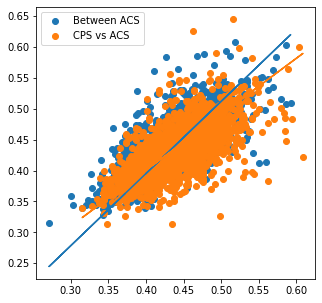
\includegraphics[scale=0.45]{images/CPS_vs_ACS.png} }
\noindent Note: The scatterplot in orange illustrates ``2000 CPS vs 2010 ACS", and the scatterplot in blue describes ``2010 ACS vs 2015 ACS". Regression lines are fitted using orthogonal least squares. They have similar distributions. 
\end{center}

Figure 3.3 shows the comparison. The similar shapes of these two scatterplots justify the comparability between the data of these two sources-- it is obvious that counties with high Gini coefficients in the CPS should have high Gini coefficients in ACS, and vice versa, so that it is reasonable to directly aggregate these two data sources. Similar results are obtained when comparing ``2000 CPS vs 2010 ACS" and ``1990 CPS vs 2000 CPS". 

\subsubsection{Other statistics}

I have also collected other statistics that help to characterize counties, in particular those concerning counties' labor force dynamics. 

These data make it possible to create a subset of comparable counties, in which each county will share similar labor force dynamics with at least some other counties. This approach will prove important since we don't want our dependent variable--individual income tax--to be substantially affected by factors outside the analysis. For example, some counties may have witnessed a large population of young people moving in, while others may see non-negligible changes in gender ratios; these changes in labor force structure may be reflected as significant disparities of individual income tax. Therefore, these labor force statistics will allow me to capture movements of taxable personal income without being substantially affected by changes beyond the business cycle. 

To construct the county population and labor force statistics, I will use the ``U.S. County Population Data - 1969-2019" from National Cancer Institute (NCI). The data represents a modification of the intercensal and Vintage 2020 annual time series of July 1, county population estimates by age, sex, race, and Hispanic origin produced by the U.S. Census Bureau's Population Estimates Program, in collaboration with the National Center for Health Statistics. From this population dataset, I extract the annual growth rates of population for 19 age groups, and compile them into growth rates for the working-age population (aged 15-64) and all population. In addition, I've also compiled the changes in gender ratio for the working-age population and all populations. These measurements should be able to provide a rough sketch of labor force dynamics for the past three decades in all U.S. counties. Finally, I have also normalized and featurized all data points so that they can later be passed into a nearest neighbor classifier to find comparable counties. 

\begin{table}[H]\centering
\renewcommand\thetable{3.4}
\caption{Summary Statistics for County Population and Labor Force Statistics}
\centerline{
    \begin{tabular}{lrrrrr}
    \toprule
    \textbf{Category} &\textbf{Variable} &  \textbf{Mean} &  \textbf{Standard} &  \textbf{Minimum} &   \textbf{Maximum} \\
    {} & {} & {} & \textbf{deviation} & {} \\
    \midrule
    {} & Percent Change in Population   &        0.0051 &      0.0166 &    -0.6553 &      0.4227 \\
    {All} & Change in Average Age   &        0.1662 &      0.1941 &    -6.6552 &      6.0389 \\
    {} & Change in Gender Ratio  &       -0.0003 &      0.0027 &    -0.1045 &      0.1550 \\
    \midrule
    {} & Percent Change in Population   &        0.0047 &      0.0191 &    -0.6670 &      0.5758 \\
    {Working-Age} & Change in Average Age   &        0.1000 &      0.1465 &    -4.1923 &      3.5911 \\
    {} & Change in Gender Ratio  &       -0.0003 &      0.0037 &    -0.1412 &      0.2027 \\
    \bottomrule
    \end{tabular}
}
\end{table}

Table 3.4 reports the summary statistics of county population and labor force statistics. Changes in average age for both the working-age population and all populations have significant variations among counties. It shows the heterogeneity of population dynamics in U.S. counties. 

To use this information about counties in nearest neighbor classification, I will standardize all data to make them have zero mean and unit variance, so each variable will contribute the same weight when finding the similar counties. 

\subsection{National Aggregate Statistics}

In addition to the county-level data, I have also prepared U.S. national personal taxable income and inequality measurements for a simple time-series analysis. 

\begin{table}[htbp]\centering
\renewcommand\thetable{3.5}
\caption{Summary Statistics for National Aggregate Statistics}
\centerline{
    \begin{tabular}{lrrrrrrrr}
    \toprule
    \textbf{Variable} &  \textbf{Mean} &  \textbf{Standard} &  \textbf{Minimum} &   \textbf{Maximum} \\
    {} & {} & \textbf{deviation} & {} \\
    \midrule
    GDP      &     8590.96 &  6346.63 &   859.95 &      21372.58 \\
    Personal Income       &     7243.75 &  5526.06 &   665.72 &      19627.58 \\
    Core PCE &       67.27 &    29.29 &    19.31 &        113.55 \\
    Gini coefficient     &        0.44 &     0.03 &     0.38 &          0.48 \\
    \bottomrule
    \end{tabular}
}
\end{table}

\subsection{ZIP Code Level Statistics}
Lastly, to provide further spatial granularity, I've compiled personal income tax data in 25,401 ZIP code areas in the United States during 2005-2012. The data is collected from the Internal Revenue Service (IRS) "SOI Tax Stats - Individual Income Tax Statistics - ZIP Code Data (SOI)". These ZIP code areas account for around 60\% of all ZIP code areas in the U.S., while the rest of ZIP code areas do not make consistent appearances in the IRS data. 

I calculated the approximate Gini coefficient for each ZIP code area by using the total tax collected and total number of exemptions (which approximates the population) in each AGI class. For each AGI class $i$, let the total individual income tax collected in that class be represented by $TAX_i$ and population be represented by $POP_i$, then we can approximate Gini-coefficient using the area under the synthetic Lorentz curve (intuitively the sum of areas of all ``trapezoids"):

$$ \hat{G} = 1 - \frac{\sum_{i}{POP_i}}{\sum_{i}{TAX_i}} \sum_{i=1}^{n}({(\sum_{j=0}^{i-1}TAX_{j} + \sum_{k=0}^{i}TAX_k) \cdot POP_i }) $$
where $ TAX_0 = 0 $

% SUMMARY STASTICS
\begin{table}[H]\centering
\renewcommand\thetable{3.6}
\caption{Summary Statistics for ZIP Code Level Statistics}
\centerline{
    \begin{tabular}{lcccc}
    \toprule
    \textbf{Variable} &  \textbf{Mean} &  \textbf{Standard} &  \textbf{Minimum} &   \textbf{Maximum} \\
    {} & {} & \textbf{deviation} & {} \\
    \midrule
    Number of returns (n1)         &    5462.29 &         6595.00 &     45.00 &  9.81e+04  \\
    Number of exemptions (n2)      &   10875.34 &        13285.18  &     92.00 &  1.35e+05 \\
    Adjusted Gross Income          &  319978.57 &       500672.33 &   2708.00 &  1.87e+07  \\
    Total income tax revenue       &   41636.83 &        89709.13 &     97.00 &  4.49e+06  \\
    Gini coefficient estimates     &       0.57 &            0.08 &     -0.39 &  0.96      \\
    Real GDP                       &   15659.07 &          317.59 &  15236.26 &  1.62e+04  \\
    \bottomrule
    \end{tabular}
}
% \begin{flushleft}
% \textbf{Notes}: \\
% \textbf{n1}: Number of returns, which approximates the number of households \\
% \textbf{n2}: Number of personal exemptions, which approximates the population \\
% \end{flushleft}
\end{table}





% ############
% MODEL 
% ############

\pagebreak
\section{Empirical Specifications}

In this section, I will provide a brief overview of the empirical specifications. A panel regression analysis will be the focus of the study, supplemented by additional time-series and cross-sectional examinations. 

\subsection{Panel Regression}

To assess the effect of income inequality on individual taxable income, I employ a panel regression model with county and year fixed effects. The model I will estimate is:

$$ \Delta \ln I_{i, t} = \bar \alpha_0 + \delta_t + \lambda_i + \theta (HighGini_{i, t} \times \Delta \ln AggregateIncome_t) + \epsilon_{i, t}$$

\begin{flushleft}
where $I_{i, t}$ is the percent change in total taxable income in county $i$ and year $t$, $\alpha_0$, $\delta_t$,  $\lambda_i$ are intercepts, and $(HighGini_{i, t}$ is the indicator variable that is 1 when a county is consider to have high Gini-coefficient (i.e. high income inequality), and 0 otherwise. $AggregateIncome_t$ is the percent change in aggregate taxable income for all counties during given year $t$. $\theta$ is the estimate for the effect of high income inequality on the dependent variable. 
\end{flushleft}

Results without county or year fixed effect will also be estimated. 

\subsection{National Aggregate Time-Series OLS}

I will also present a simple OLS setup with national aggregate data to show if growing income inequality has resulted in increased cyclicality of tax revenue on a national level. In addition, this will also help to verify the pro-cyclicality of individual taxable income. The model I will estimate is:

$$ \Delta \ln I_t = \bar \alpha_0 + \theta_0 \Delta \ln Y_t + \theta_1 (\Delta \ln Y_t \times Gini_t) + \epsilon_{t}$$

\begin{flushleft}
where $I_{i, t}$ is the percent change in total taxable income year $t$, $\alpha_0$ is the intercept, $\Delta Y_t$ is the percent growth of GDP in year $t$, $Gini$ is the Gini-coefficient. 
\end{flushleft}









% ############
% RESULTS 
% ############

\pagebreak
\section{Results}


\subsection{National Aggregate Time Series}
In this section, I will use the national aggregate data from 1969 to 2020 and conduct a basic time series analysis. 
% NATIONAL AGGREGATE TIME SERIES VISUALIZATION
\begin{center}
Figure 5.1: Historical Trend of GDP, Personal Income, and Income Inequality as Measured by Gini Coefficient, 1968-2020
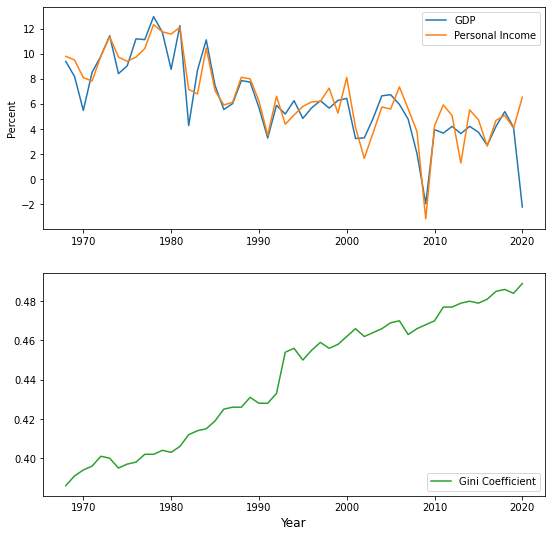
\includegraphics[scale=0.5]{images/historical_time_series.png}
\end{center}

Figure 5.1 shows the movements of gross domestic product(GDP), personal taxable income, and the income inequality measure during this period. Personal taxable income moved very closely with output, while the income inequality increased steadily over time. It does appear the personal income fluctuates more recently than in the past, especially beginning 2010. 

\vspace{5mm}

Next, I will explore the relationship between national aggregate personal taxable income and aggregate output (GDP), and test if the growing income inequality represented by Gini Coefficient may have contributed to the growing volatility. 

% NATIONAL AGGREGATE TIME SERIES REGRESSION
\begin{table}[htbp]\centering
\renewcommand\thetable{5.2}
\caption{Dependent Variable: Change in Personal Taxable Income}
\centerline{
    \begin{tabular}{l c c}
    \toprule
    \textbf{}                          & \textbf{(A)}     & \textbf{(B)} \\ 
    \textbf{Variable}                  & \textbf{Nominal} & \textbf{Real}\\
    \midrule
    intercept                          &       0.0096     &  0.0075      \\
                                       &      (0.012)     & (0.005)      \\
    change in GDP                      &       1.3709**   &  0.5780      \\
                                       &      (0.694)     & (0.641)      \\
    change in GDP $\times$             &       -1.1324    &  0.5362      \\
    {         Gini coefficent}         &      (1.984)     & (1.670)      \\
    \midrule
    \textbf{$R^2$}                     &       0.855      &  0.694       \\
    N. of Observations                 &       52         &  52          \\         
    \bottomrule
    \addlinespace[1ex]
    \multicolumn{3}{l}{\textsuperscript{***}$p<0.01$, 
      \textsuperscript{**}$p<0.05$, 
      \textsuperscript{*}$p<0.1$}
    \end{tabular}
}
\end{table}

Table 5.2 reports the OLS regression results for national aggregate time series analysis. Column (A) uses nominal variables (i.e. nominal GDP, nominal personal income). As expected the change in personal taxable income has a strong correlation with the change in GDP--personal taxable income will increase 1.37\% for every 1\% increase in aggregate output. However, the estimated effect of income inequality is not significant, and it seems the trend of personal taxable income cannot be explained by the increasing income inequality. Column (B) uses real variables (nominal variables adjusted by price level). Neither results are significant. 

\pagebreak







\subsection{County Panel}
In order to explore how income inequality has influenced tax revenue cyclicality more closely, we will then examine county level data starting from 1989. Cross-sectional comparisons of how regional income tax revenue reacts to the business cycle may answer our question--whether higher income inequality can result in a higher level of tax revenue cyclicality. We will continue to use the total personal taxable income (or the tax base) in each county as the key dependent variable. 

\subsubsection{Basic Setup}

This section will present the results of panel analysis using county level taxable income data from 1989 to 2019. In the county level income data obtained from the Internal Revenue Service (IRS), it contains data of aggregate gross income (AGI), wages and salaries, taxable dividend income, and taxable interest income for each county. 

In the following panel data analysis, I will first explore how the overall county income (represented by AGI) change in high income inequality counties versus low income inequality counties, and then move on to examine the dynamics of county income of each source (wages and salaries, dividend income, or interest income) in high versus low income inequality counties. 

% Regression result for Basic Panel Setup (Overall)
\begin{table}[htbp]
\renewcommand\thetable{5.3}
\caption{Dependent Variable: Change in Personal Taxable Income}
\centerline{
    \begin{tabular}{l c c c c}
    \toprule
    \textbf{} & \textbf{(A)} & \textbf{(B)} & \textbf{(C)} & \textbf{(D)}\\ 
    \textbf{Variable} & \textbf{Pooled} & \textbf{Cross-section} & \textbf{Time-series} & \textbf{Two-way fixed} \\
    \midrule
    intercept                          &       3.8546*** &  3.7927***  &       4.1719*** &  4.1121***\\
                                       &      (0.0436)   & (0.0461)    &      (0.0364)   & (0.0370)\\
    change in aggregate income         &       0.2035*** &  0.2388***  &       0.0225***    &  0.0566***\\
    {$\times$ high income inequality}  &      (0.0095)   & (0.0115)    &      (0.0085)   & (0.0085)\\
    \midrule
    Time fixed effect                  &       No        &  Yes        &       No        &  Yes        \\
    ZIP code fixed effect              &       No        &  No         &       Yes       &  Yes        \\
    \midrule
    \textbf{$R^2$}                     &       0.0355    &  0.0467     &       0.0003    &  0.0019\\
    N. of Observations                 &       23280     &  23280      &       23280     &  23280 \\         
    \bottomrule
    \addlinespace[1ex]
    \multicolumn{3}{l}{\textsuperscript{***}$p<0.01$, 
      \textsuperscript{**}$p<0.05$, 
      \textsuperscript{*}$p<0.1$}
    \end{tabular}
}
\end{table}

Table 5.3 reports the results of the panel analysis. The pooled panel regression captures the general trend--personal taxable income in counties with high income inequality are more exposed to business cycle than the national average by 0.20\%. When accounting for the time fixed effect, the average estimated effect of high income inequality increases to 0.24\%. However, when adding in ZIP code effects, the estimated effect of high income inequality decreases. With only the ZIP code effect included, high income inequality has a less substantial effect on taxable income sensitivity. When I include both ZIP code effect and time fixed effect, the estimated effect is highly significant, but the coefficient has reduced to 0.057\%. 

From a cross-sectional perspective, it looks like higher income inequality is indeed linked to a higher sensitivity of taxable income with respect to the business cycle; however, the relationship is much less robust from a time-series perspective. This is in line with the previous national aggregate analysis, which shows a less significant association between higher income inequality and higher income sensitivity. 

\vspace{5mm}

In the following analysis, I will attempt to explain why the overall panel regression results behave in this way. In particular, I suspect the relationship may be heterogeneous for different time periods and income of different sources, so I will break down the data both by time and by income source, and examine the correlation for each. 

First, I will construct a Two-Way Fixed Effect model for personal income by different sources. Since the taxable income data from IRS only contains consistent observations for personal income of three sources from 1989-2019, I will break down all the data into these three categories (wages and salaries, dividend income, interest income). However, it is worth to note that other important income sources such as capital gains may provide crucial information, and would have been another focus of this analysis if consistent data from 1989-2019 were available. 


% REGRESSION
\begin{table}[htbp]\centering
\renewcommand\thetable{5.4}
\caption{Dependent Variable: Change in Personal Taxable Income by Source}
\centerline{
    \begin{tabular}{l c c c c}
    \toprule
    \textbf{} & \textbf{(A)} & \textbf{(B)} & \textbf{(C)} & \textbf{(D)}\\ 
    \textbf{Variable} & \textbf{Overall} & \textbf{Wages} & \textbf{Dividends} & \textbf{Interest}  \\
    \midrule
    intercept                          &       4.1121*** &  3.9136***  &       5.3377*** & -1.7468\\
                                       &      (0.0370)   & (0.0308)    &      (0.0996)   & (0.0580) \\
    change in aggregate income         &       0.0566***&  0.0321*** &       0.0010    &  0.0657***  \\
    {  $\times$ high income inequality}  &      (0.0085)   & (0.0100)    &      (0.0145)   & (0.0090) \\
    \midrule
    Time fixed effect                  &       Yes       &  Yes        &       Yes       &  Yes     \\
    ZIP code fixed effect              &       Yes       &  Yes        &       Yes       &  Yes     \\
    \midrule
    \textbf{$R^2$}                     &       0.0355 &  0.0003     &       3.37e-07    &  0.0035\\
    N. of Observations                 &       23280     &  23280      &       23280     &  23280   \\         
    \bottomrule
    \addlinespace[1ex]
    \multicolumn{3}{l}{\textsuperscript{***}$p<0.01$, 
      \textsuperscript{**}$p<0.05$, 
      \textsuperscript{*}$p<0.1$}
    \end{tabular}
}
\end{table}

Table 5.4 reports the results. When breaking down personal income by the income source, we can observe an interesting pattern. Income from all four sources shows a greater cyclicality when income inequality is higher. Wages and salaries and taxable interest income behave similarly to overall personal income--a county with high income inequality tends to experience 0.057\% and 0.066\% more cyclical movement respectively with respect to the national aggregate wages and salaries. The estimated effect is highly significant. On the other hand, even though the effects are insignificant, taxable dividend income exhibits 0.001\% more cyclical movement on average. 

Even though the coefficient estimates for dividend income are not significant, this analysis still helps to clarify the underlying heterogeneity of income of different sources. 

\vspace{5mm}

In the next step, I will take a look at whether similar heterogeneity exists in personal income of different time periods. To do this, we will use subsets of data and evaluate the same panel regression setup as above. 

% SUBSET RESULTS




\begin{center}
Figure 5.5: Estimated Coefficients for ``Change in Aggregate Income $\times$ High Income Inequality" Using 10-year Subsets for Total Income and Income of Different Sources\\
\noindent
\makebox[\textwidth]{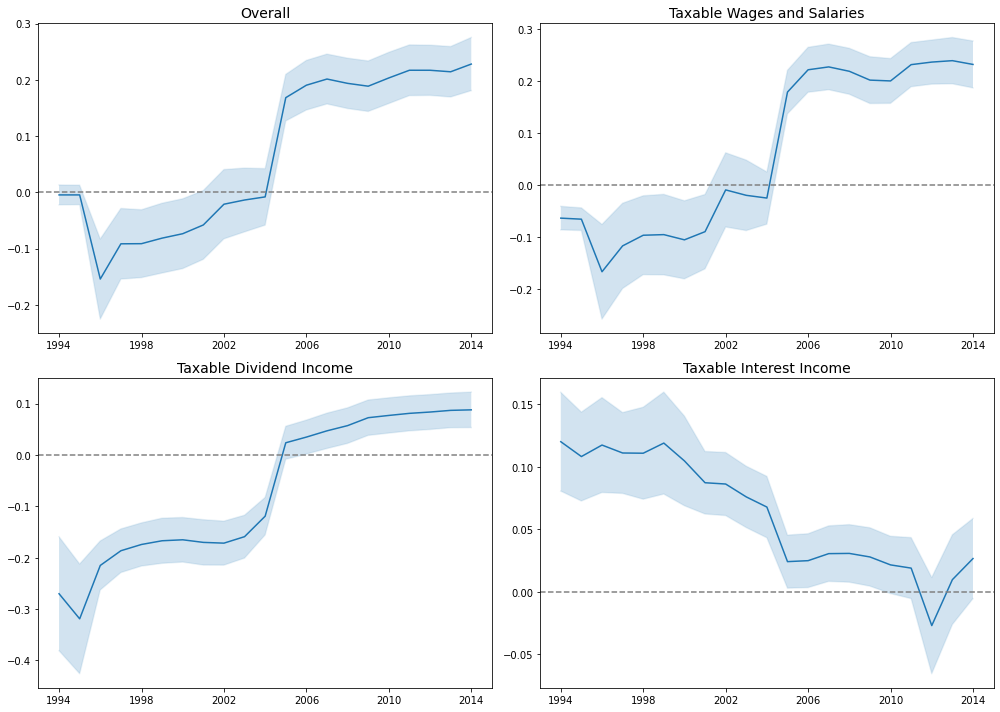
\includegraphics[scale=0.45]{images/county_basic/panel_subset_basic_1.3.png}}

Note: The estimated coefficients are obtained by performing panel regression with TWFEs on 10-year subsets of county-level data. The horizontal axis specifies the time period for each data subset, where the number represents the "middle"s of 10-year subsets. The bands around the curves are the standard error margins (or 95\% confidence intervals).
\end{center}

The above figures (Figure 5.5) illustrate the regression result coefficients for ``change in aggregate income $\times$ high income inequality" using 10-year subsets of data. For example, 2004 on the horizontal axis means the corresponding regression estimate is obtained by using a subset with data from 1999-2009. The solid blue curves are the regression estimates for each subsets. The figures demonstrate the evolution of the estimated effect of income inequality on personal income cyclicality. 

The first figure (Overall income) shows negative effects before around 2003 and positive significant effects after 2003--on average high income inequality counties experience 0.2\% more increase than low income inequality counties when the national aggregate income grows by 1\% starting around 2005-2006. Wages and salaries have undergone similar dynamics in the past 30 years. 

For taxable dividend income, the effect also went from negative to positive around 2004-2005, and the historical trend of the estimated effects over the past three decades agrees with the overall income. Interestingly, taxable dividend income appears to have less cyclicality when income inequality is high. It is also important to note that personal income from capital gain closely resembles dividend income on a national scale, so it may suggest income inequality shares a similar trend over the past thirty years on these two sources of income. 

Taxable interest income does not show a significant estimated effect with any subsets, though the estimated effects have dropped from positive to zero.

\begin{center}
Figure 5.6: Composition of Income Before Transfers Among the Top 1 Percent Income Household, 1978 to 2018\\
\noindent
\makebox[\textwidth]{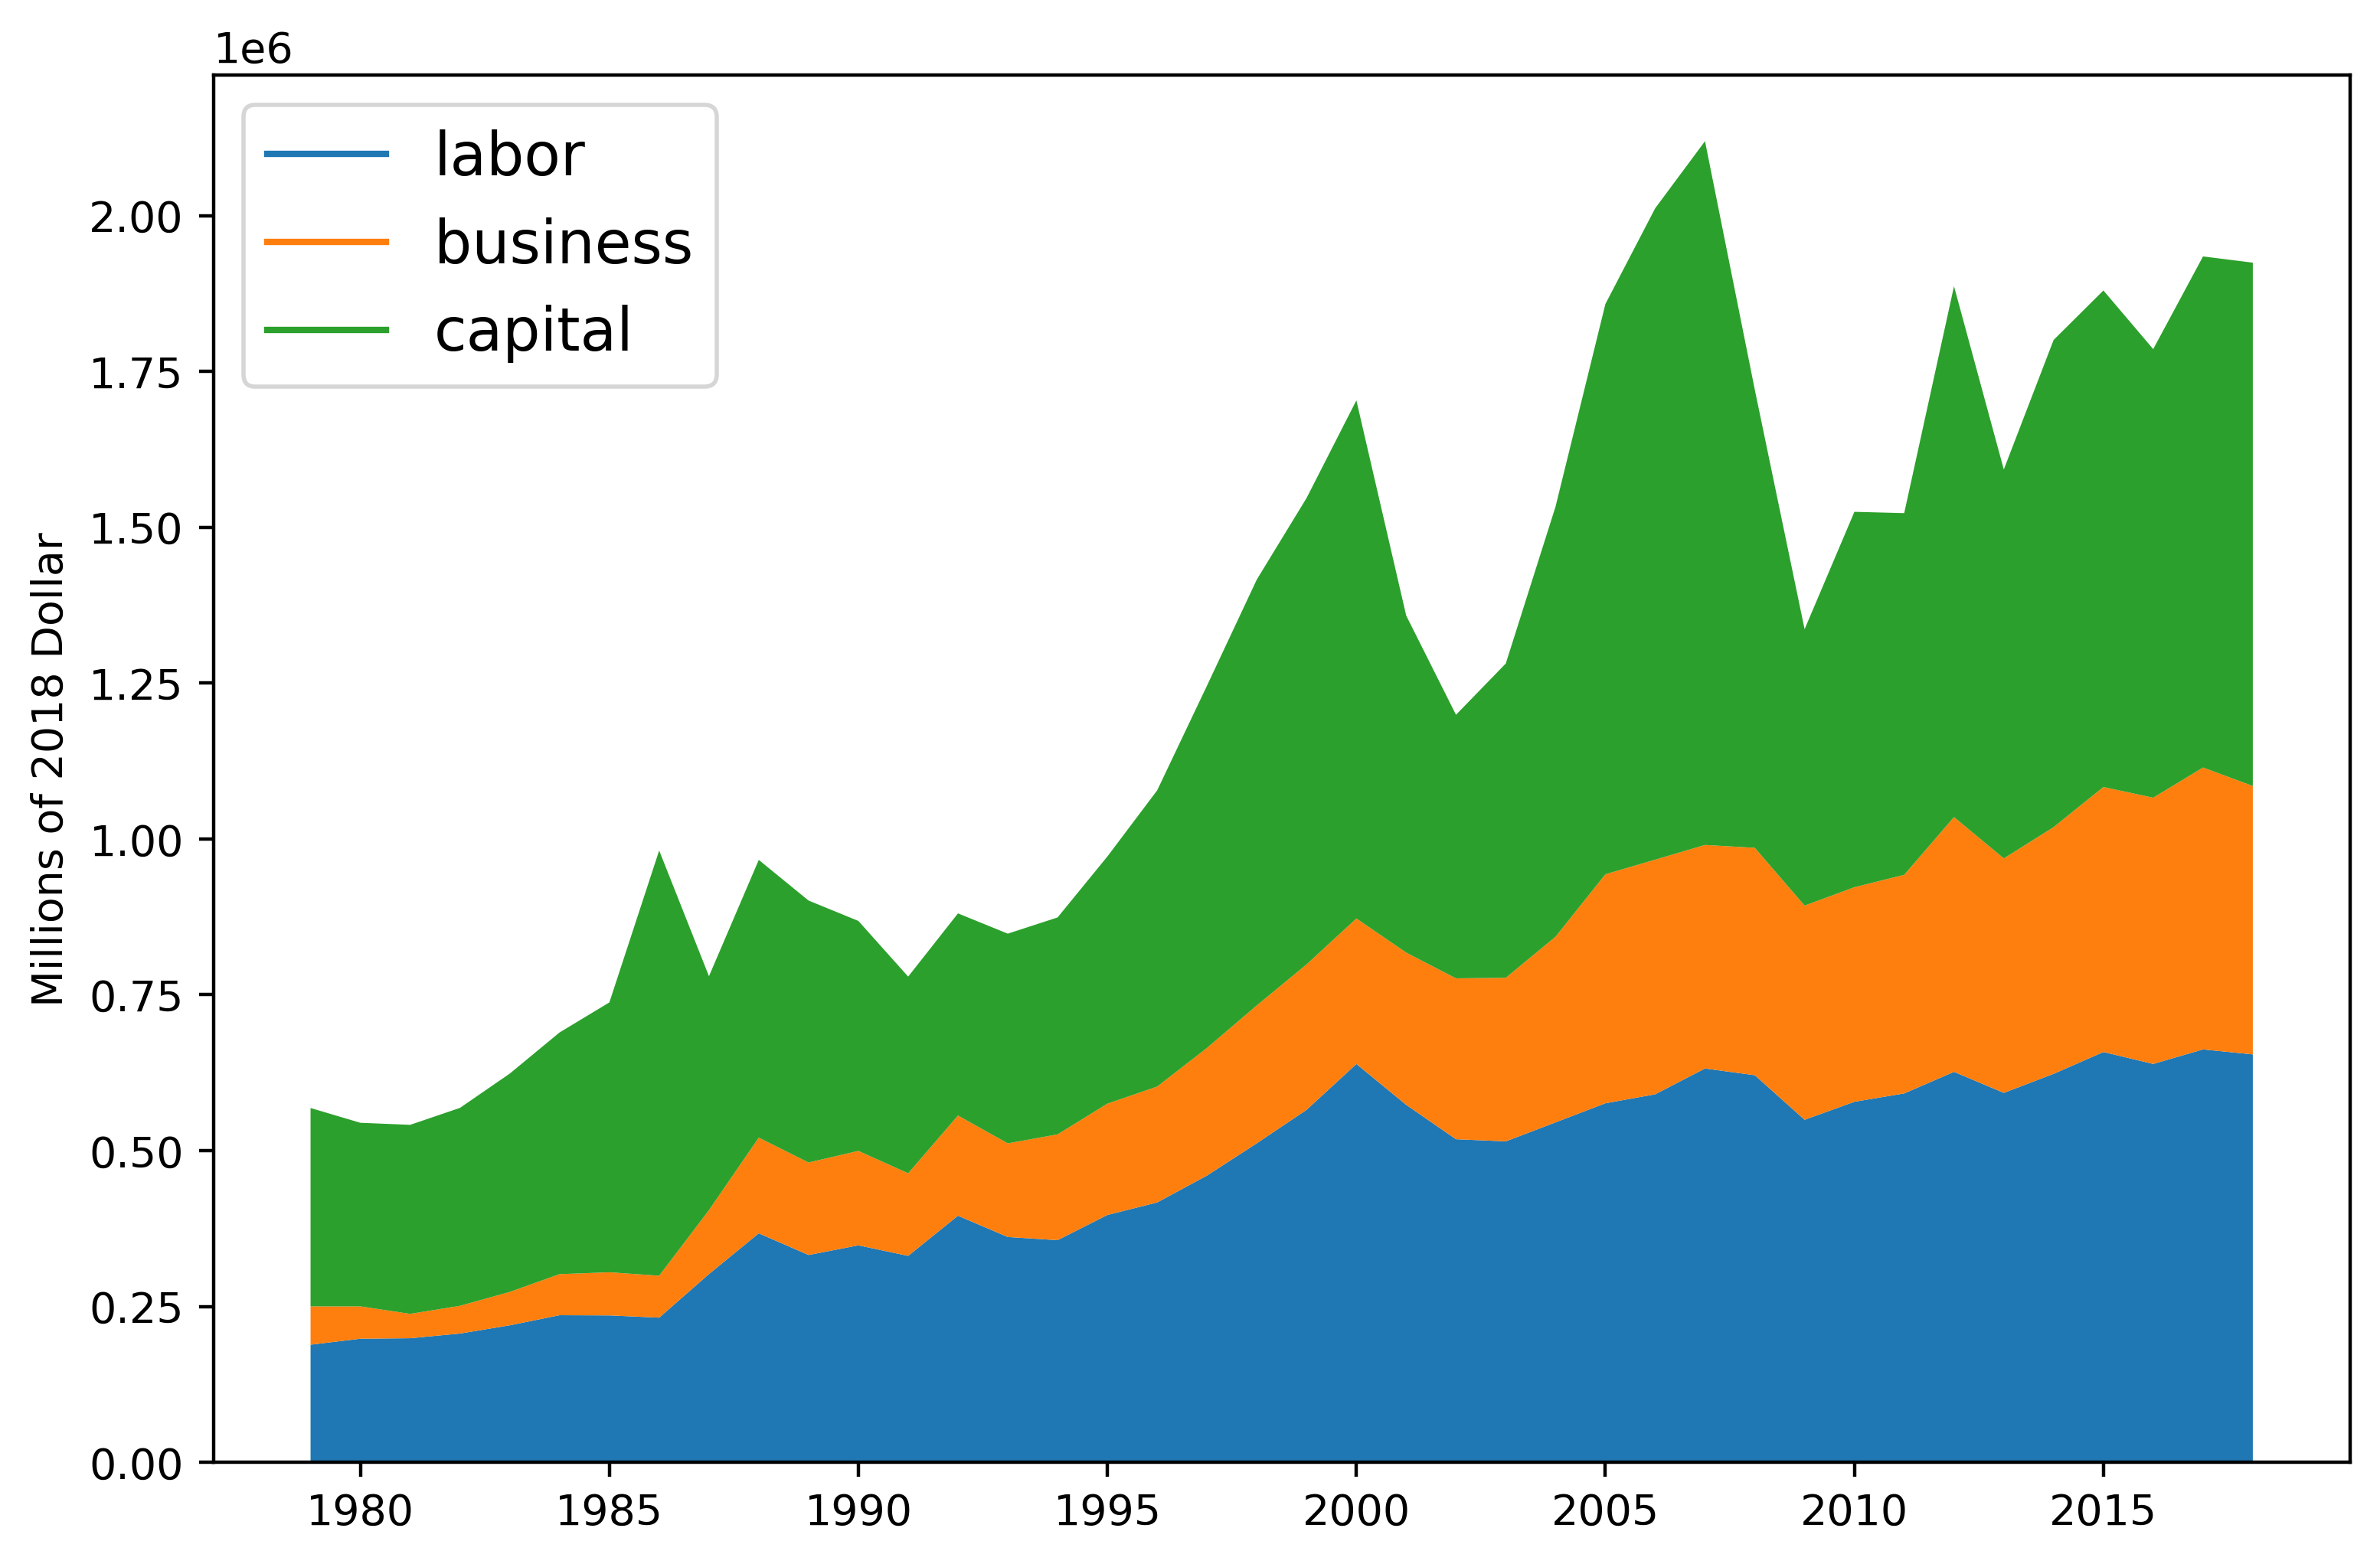
\includegraphics[scale=0.4]{images/county_basic/income_composition.png}}
Source: Piketty and Saez (2003) and Congressional Budget Office (2021)
\end{center}

One possible explanation for the above dynamics of the estimated effect of income inequality on personal taxable income by different sources may be the evolution of income composition, particularly for the top income population. Piketty and Saez (2003) put together data for top 0.1 percent income share and composition, and discovered a significant increase of capital gain as part of the total income, especially when the economy is booming. 

Figure 5.6 illustrates how each income component has grown over time for the top income households. As the overall share of income for top 1 percent income households increases, Piketty and Saez (2006) attributed this rise not to the revival of top ``traditional" capital incomes, but rather to the very large increases in top wages (especially top executive compensation) and capital gains. ``top executives (the “working rich”) replaced top capital
owners (the “rentiers”) at the top of the income". 

Wages and salaries, interest income, rents, royalties used to make up a higher proportion of income for the top income group; starting early 2000, capital gains and business income gradually played a more significant role. Giertz and Mortenson (2013) used Execucomp executive income to further decompose capital income, and discovered how stock options, stock awards, bonuses, and non-equity incentive plan compensation (non-equity Inc) are tightly associated with increased volatility of income of top executives. In particular, the authors noted that ``despite [stock option value] rising in absolute terms by 363 percent from 1992 to 2000 and by 127 percent from 2002 to 2006, the value of stock options was up just 55.9 percent on net from 1992 to 2010. From 2000 to 2010, their value fell by 33.7 percent, on net." 

The rising share of capital gains and business income for higher income populations make their income highly correlated with the overall performance in the economy and also in the business and financial markets, thus may have exposed their personal income more to the business cycle. Also the increasingly important bonus (which behaves closer to stock options than salaries) may also have contributed to rising cyclicality of personal income. These help to explain the positive significant effect of income inequality on overall personal income, wages and salaries, and dividend income starting this century, and the declining effect of income inequality on interest income. 


\pagebreak






\subsubsection{Nearest Neighbor Matching}

Counties and counties are different. The past three decades have witnessed dramatic changes both demographically and economically to counties that should be accounted for. 

Thus, it is essential to make sure the analysis is comparing apples with apples, and that any differences between personal income changes among high versus low income inequality counties are not affected substantially by changes beyond the business cycle. To do this, I will use nearest neighbor matching (similar to propensity score matching) to match each high income counties to the 3 most similar low income counties, based on demographic characteristics, including population, working age population, gender distribution over the past three decades as the primary features. 

I will then use data for all the high income inequality counties and all the \textit{matched} low income inequality counties to perform the panel regression analysis. Using matching helps to eliminate counties that are not comparable to any other counties, so that the result is more reliable. 

\vspace{5mm}

\begin{table}[htbp]\centering
\renewcommand\thetable{5.7}
\caption{Dependent Variable: Change in Personal Taxable Income}
\centerline{
    \begin{tabular}{l c c c c}
    \toprule
    \textbf{} & \textbf{(A)} & \textbf{(B)} & \textbf{(C)} & \textbf{(D)}\\ 
    \textbf{Variable} & \textbf{Pooled} & \textbf{Cross-section} & \textbf{Time-series} & \textbf{Two-way fixed} \\
    \midrule
    intercept                          &       3.5394*** &  3.4930***  &       3.9598*** &  3.9102***\\
                                       &      (0.0511)   & (0.0542)    &      (0.0411)   & (0.0435)\\
    change in aggregate income         &       0.2186*** &  0.2388***     &       0.0353*** &  0.0569***\\
    {  $\times$ high income inequality}  &      (0.0101)   & (0.0115)    &      (0.0090)   & (0.0089)\\
    \midrule
    Time fixed effect                  &       No        &  Yes        &       No        &  Yes        \\
    ZIP code fixed effect              &       No        &  No         &       Yes        &  Yes        \\
    \midrule
    \textbf{$R^2$}                     &       0.0530    &  0.0618     &       0.0008    &  0.0017\\
    N. of Observations                 &       17790   &  17790    &       17790   &  17790 \\         
    \bottomrule
    \addlinespace[1ex]
    \multicolumn{3}{l}{\textsuperscript{***}$p<0.01$, 
      \textsuperscript{**}$p<0.05$, 
      \textsuperscript{*}$p<0.1$}
    \end{tabular}
}
\end{table}

Table 5.7 reports the panel regression results using nearest neighbor matched counties. The results agree with the previous regression results without matching, but the time-series analysis using matched county data shows highly significant results. However, the estimated effect remains small compared with the cross-sectional examination. 

\pagebreak

Similarly, I will also break down the data by time period and by sources of income to account for the heterogeneity. 

% REGRESSION
\begin{table}[htbp]\centering
\renewcommand\thetable{5.8}
\caption{Dependent Variable: Change in Personal Taxable Income by Source}
\centerline{
    \begin{tabular}{l c c c c}
    \toprule
    \textbf{} & \textbf{(A)} & \textbf{(B)} & \textbf{(C)} & \textbf{(D)}\\ 
    \textbf{Variable} & \textbf{Overall} & \textbf{Wages} & \textbf{Dividends} & \textbf{Interest}  \\
    \midrule
    intercept                          &       3.9102*** &  3.6821***  &       5.1591*** & -1.8205***\\
                                       &      (0.0435)   & (0.0373)    &      (0.1207)   & (0.0671) \\
    change in aggregate income &       0.0569***&  0.0362*** &       0.1015***  &  0.0661***  \\
    {  $\times$ high income inequality}  &      (0.0089)   & (0.0107)    &      (0.0163)   & (0.0100) \\
    \midrule
    Time fixed effect                  &       Yes       &  Yes        &       Yes       &  Yes     \\
    ZIP code fixed effect              &       Yes       &  Yes        &       Yes       &  Yes     \\
    \midrule
    \textbf{$R^2$}                     &       0.0017 &  0.0004     &       1.474e-05 &  0.0031\\
    N. of Observations                 &       17790     &  17790      &       17790     &  17790   \\         
    \bottomrule
    \addlinespace[1ex]
    \multicolumn{3}{l}{\textsuperscript{***}$p<0.01$, 
      \textsuperscript{**}$p<0.05$, 
      \textsuperscript{*}$p<0.1$}
    \end{tabular}
}

\end{table}

Table 5.8 reports the results using matched data. These results are in line with the previous finding. However, with popular and labor force dynamics matched county data, the estimated effects are being more significant. In particular, the wages and salaries now show a highly significant interaction with income inequality as measured by Gini coefficients--counties with high income inequality typically see 0.03\% more increase than average when the aggregate income for each income source increases by 1\%. Still, the coefficient for dividend income remains insignificant. 

I have also run regression with 10-year subsets using the same approach as in the previous basic setup. The regression results are showing much smaller error margins using the nearest neighbor matched data. The trend, on the other hand, stays the same as before. 

\pagebreak

\begin{center}
Figure 5.9: Estimated Coefficients for ``Change in Aggregate Income $\times$ High Income Inequality" Using 10-year Subsets for Total Income and Income of Different Sources (Nearest Neighbor Matched Counties)\\
\noindent
\makebox[\textwidth]{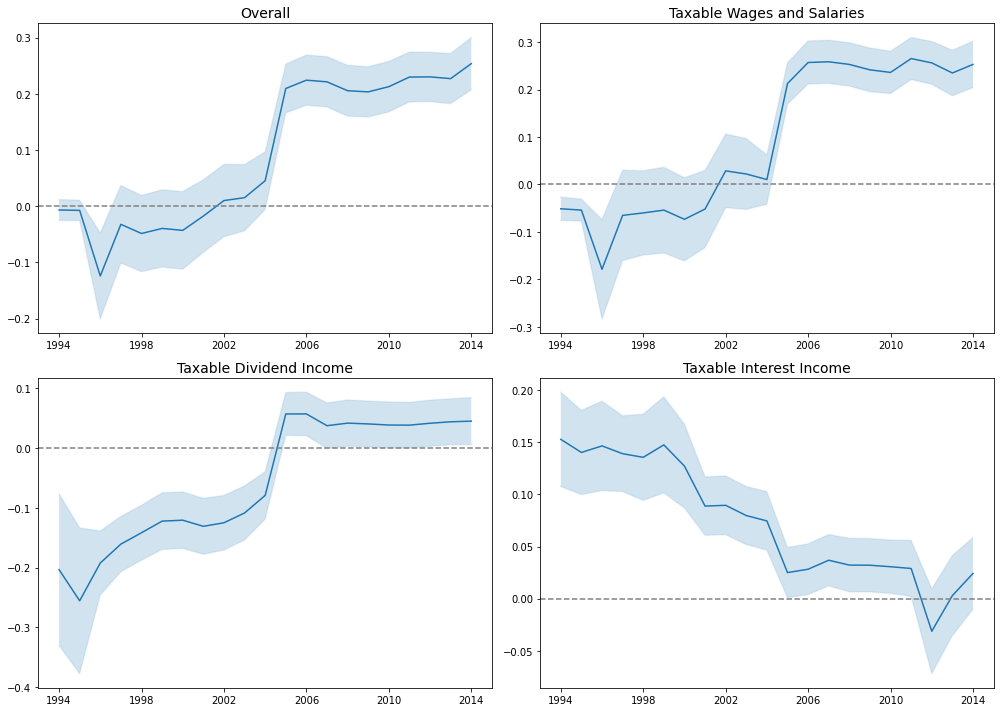
\includegraphics[scale=0.45]{images/county_matched/panel_subset_matched_1.3.png}}
Note: The estimated coefficients are obtained by performing panel regression with TWFEs on 10-year subsets of county-level nearest neighbor matched data. The horizontal axis specifies the time period for each data subset, where the number represents the "middle"s of 10-year subsets. The bands around the curves are the standard error margins (or 95\% confidence intervals).
\end{center}

% \subsubsection{Discussion}

\pagebreak

\subsection{Results from ZIP Code Areas (2005-2012)}
In this section, I will present the results of difference-in-difference analysis using ZIP Code level data from 2005-2012. 

% VISUALIZATION
\begin{center}
Figure 5.10: Total Personal Income Tax Changes in High vs Low Income Inequality Areas
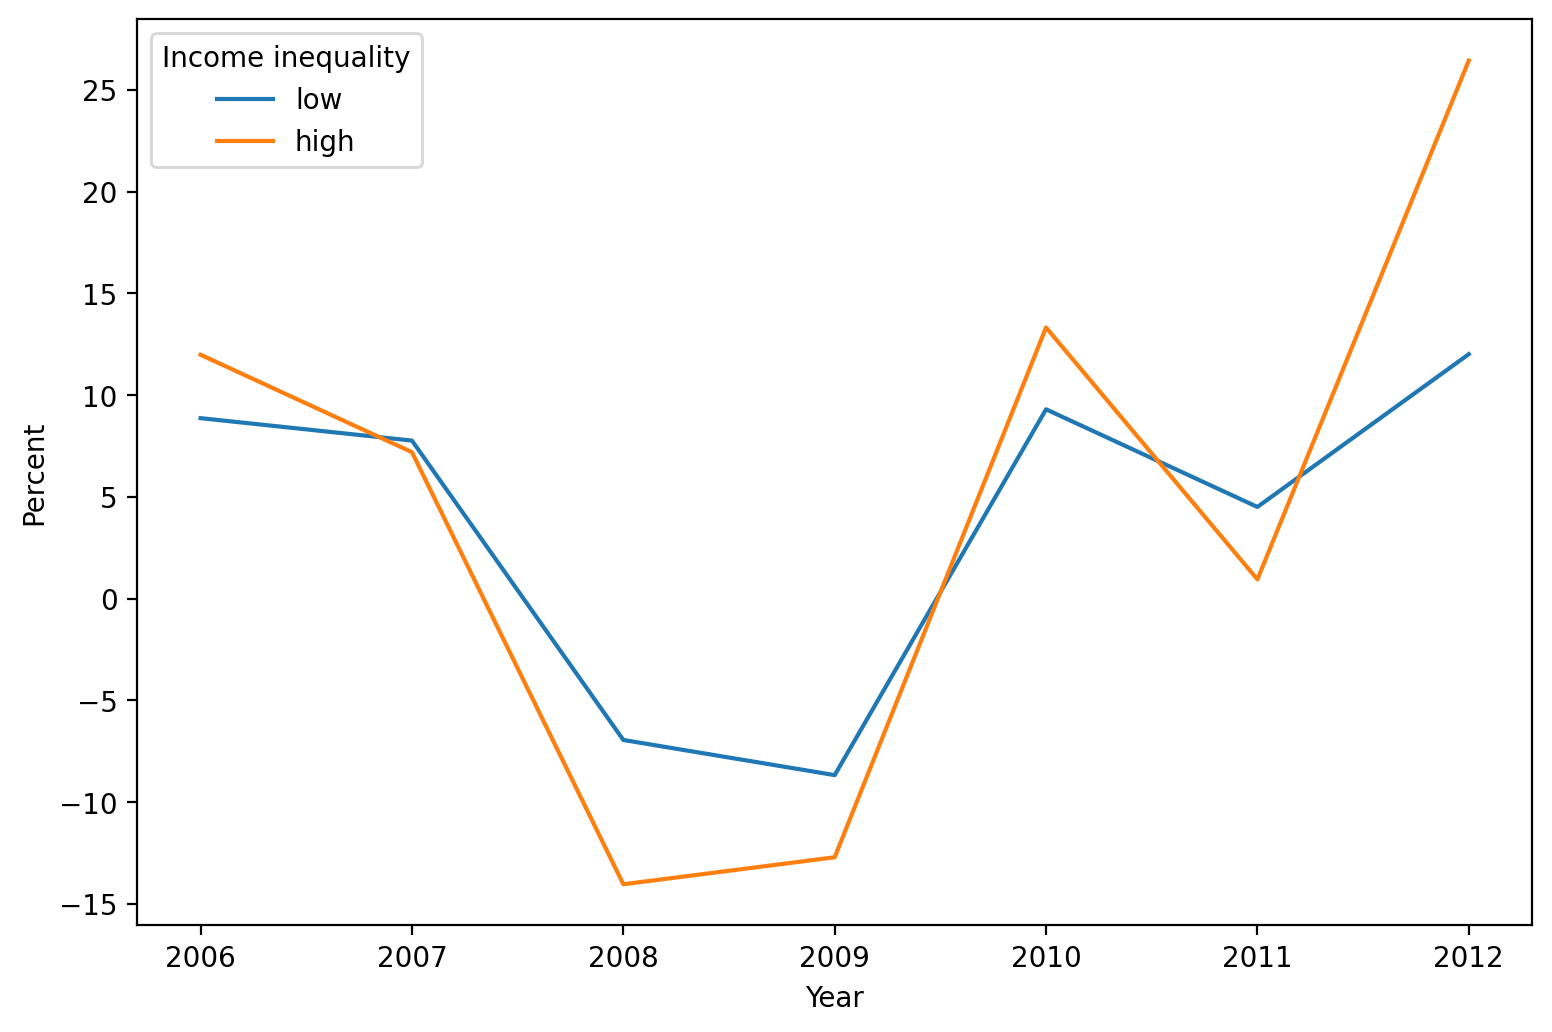
\includegraphics[scale=0.5]{images/high_vs_low_gini.png}
\end{center}

In Figure 5.10, I take the ZIP code areas with the highest Gini coefficient and compare them against the rest. It is pretty clear that in places with higher income inequality, the personal income tax revenue responds more to the business cycles. During the GFC, ZIP code areas with the highest income inequality suffered on average around 5\% more decline in personal income tax revenue. \\


% REGRESSION
\begin{table}[htbp]\centering
\renewcommand\thetable{5.11}
\caption{Dependent Variable: Percentage Change in Income Tax Revenue}
\begin{tabular}{l c c}
\toprule
\textbf{} & \textbf{(A)} & \textbf{(B)} \\ 
\textbf{Variable} & \textbf{Pooled} & \textbf{Cross-section} \\
\midrule
intercept                          &       1.4714*** &  1.4714***  \\
                                   &      (0.0803)   & (0.0865)    \\
change in real GDP                 &       2.6642*** &  2.6722***  \\
                                   &      (0.0331)   & (0.0371)    \\
change in real GDP $\times$        &       1.6109*** &  0.8104     \\
{         high income inequality}  &      (0.4234)   & (0.6696)    \\
\midrule
Time fixed effect                  &       No        &  Yes        \\
ZIP code fixed effect              &       No        &  No         \\
\midrule
\textbf{$R^2$}                     &       0.0195    &  0.0195     \\
N. of Observations                 &       175,284   &  175,284    \\         
\bottomrule
\addlinespace[1ex]
\multicolumn{3}{l}{\textsuperscript{***}$p<0.01$, 
  \textsuperscript{**}$p<0.05$, 
  \textsuperscript{*}$p<0.1$}
\end{tabular}
\end{table}

Table 5.11 reports the regression results on ZIP code area level. For every 1\% increase in the real GDP, the personal income tax revenue is expected to increase by 2.66\%. For those ZIP code areas with highest income inequality, the change in tax revenue is about 4.27\% per 1\% change in real GDP. 

In addition, even though the overall R-squared is low, the model gives a very high ``Between R-square". This indicates the model is capable of capturing the variation in the change in tax revenue between the ZIP code areas. This aligns with the previous panel regression results that the cross-sectional estimated effects appear more significant. 

% REGRESSION
\begin{table}[htbp]\centering
\renewcommand\thetable{5.12}
\caption{Dependent Variable: Percentage Change in Income Tax Revenue}
\begin{tabular}{l c c}
\toprule
\textbf{} & \textbf{(A)} & \textbf{(B)} \\ 
\textbf{Variable} & \textbf{Pooled} & \textbf{Cross-section} \\
\midrule
intercept                          &       2.3090*** &  2.3090***  \\
                                   &      (0.0763)   & (0.0801)    \\
change in aggregate tax revenue    &       0.6590*** &  0.6603***  \\
                                   &      (0.0077)   & (0.0084)    \\
change in aggregate tax revenue $\times$        &       0.5183*** &  0.3857***     \\
{         high income inequality}  &      (0.1083)   & (0.1393)    \\
\midrule
Time fixed effect                  &       No        &  Yes        \\
ZIP code fixed effect              &       No        &  No         \\
\midrule
\textbf{$R^2$}                     &       0.0194    &  0.0225     \\
N. of Observations                 &       175,284   &  175,284    \\         
\bottomrule
\addlinespace[1ex]
\multicolumn{3}{l}{\textsuperscript{***}$p<0.01$, 
  \textsuperscript{**}$p<0.05$, 
  \textsuperscript{*}$p<0.1$}
\end{tabular}
\end{table}
\pagebreak


\subsection{Robustness}
This section will examine if the above results are robust.

Previously I have defined the high income inequality regions to be those at the top 20\%, and the low income inequality inequality regions to be those at the bottom 20\%. Here we will introduce more ``cutoff"s of how high and low income inequality are defined, and test if the result will be different from the original one. 

\subsubsection{Income Inequality Cutoffs}
To test if different cutoffs have any substantial impact on the regression result, I will use two additional cutoffs for high versus low income inequality, and conduct panel analysis using the same setup as before. 

% \vspace{5mm}

First we will set the cutoff for high versus low income inequality counties to be 50\%, so that half of the counties will belong to the high income inequality group, and the rest will belong to the low inequality group.  

\begin{table}[htbp]\centering
\renewcommand\thetable{5.12}
\caption{Dependent Variable: Change in Personal Taxable Income by Source}
\centerline{
    \begin{tabular}{l c c c c}
    \toprule
    \textbf{} & \textbf{(A)} & \textbf{(B)} & \textbf{(C)} & \textbf{(D)}\\ 
    \textbf{Variable} & \textbf{Overall} & \textbf{Wages} & \textbf{Dividends} & \textbf{Interest}  \\
    \midrule
    intercept                          &       4.1547*** &  3.9348***  &       5.2714*** & -1.7731**\\
                                       &      (0.0229)   & (0.0188)    &      (0.0612)   & (0.0358) \\
    change in aggregate income         &       0.0355***&  0.0186*** &       -0.0030  &  0.0368  \\
    {  $\times$ high income inequality}&      (0.0051)   & (0.0061)    &      (0.0090)   & (0.0055) \\
    \midrule
    Time fixed effect                  &       Yes       &  Yes        &       Yes       &  Yes     \\
    ZIP code fixed effect              &       Yes       &  Yes        &       Yes       &  Yes     \\
    \midrule
    \textbf{$R^2$}                     &       0.0008    &  0.0001        &       3.762e-06 &  0.0011\\
    N. of Observations                 &       58230     &  58230      &       58230     &  58230   \\         
    \bottomrule
    \addlinespace[1ex]
    \multicolumn{3}{l}{\textsuperscript{***}$p<0.01$, 
      \textsuperscript{**}$p<0.05$, 
      \textsuperscript{*}$p<0.1$}\\
    \end{tabular}
}
\begin{flushleft}
\textit{Note:} High income inequality = 1 for counties with top 50\% Gini coefficient; high income inequality = 0 for counties with bottom 50\% Gini coefficient.
\end{flushleft}
\end{table}

Table 5.12 reports the panel regression results using the 50\% cutoff. There are no substantial changes in any coefficient estimates except the estimated effects of high income inequality on dividend income and interest income are no longer significant. This is reasonable since using the 50\% cutoff implies throwing more counties that neither have a very high or very low income inequality into the analysis, reducing the overall difference between two groups in comparison.  

Full results including results for subsets by time periods can be found in Appendix C. They also do not display any significant changes to the original results. 

\vspace{5mm}

Next we will set the cutoff for high versus low income inequality counties to be 10\%, so that the counties with top 10\% Gini coefficients will belong to the high income inequality group, and those with bottom 10\% will belong to the low inequality group.  

\begin{table}[htbp]\centering
\renewcommand\thetable{5.13}
\caption{Dependent Variable: Change in Personal Taxable Income by Source}
\centerline{
    \begin{tabular}{l c c c c}
    \toprule
    \textbf{} & \textbf{(A)} & \textbf{(B)} & \textbf{(C)} & \textbf{(D)}\\ 
    \textbf{Variable} & \textbf{Overall} & \textbf{Wages} & \textbf{Dividends} & \textbf{Interest}  \\
    \midrule
    intercept                          &       4.1468*** &  3.9376***  &       5.3516*** & -1.6404\\
                                       &      (0.0538)   & (0.0457)    &      (0.1401)   & (0.0850) \\
    change in aggregate income         &       0.0574***&  0.0186 &       0.0172    &  0.0593***  \\
    {  $\times$ high income inequality}  &      (0.0125)   & (0.0149)    &      (0.0207)   & (0.0126) \\
    \midrule
    Time fixed effect                  &       Yes       &  Yes        &       Yes       &  Yes     \\
    ZIP code fixed effect              &       Yes       &  Yes        &       Yes       &  Yes     \\
    \midrule
    \textbf{$R^2$}                     &       0.0018 &  0.0001     &       0.0001    &  0.0026\\
    N. of Observations                 &       11640     &  11640      &       11640     &  11640   \\         
    \bottomrule
    \addlinespace[1ex]
    \multicolumn{3}{l}{\textsuperscript{***}$p<0.01$, 
      \textsuperscript{**}$p<0.05$, 
      \textsuperscript{*}$p<0.1$}
    \end{tabular}
}
\begin{flushleft}
\textit{Note:} High income inequality = 1 for counties with top 10\% Gini coefficient; high income inequality = 0 for counties with bottom 10\% Gini coefficient.
\end{flushleft}
\end{table}

Table 5.13 reports the panel regression results using the 10\% cutoff.  The overall trend remains the same as the original regression results. It is interesting to observe the estimated effect for dividend income has become more significant while the estimated effects for interest income less significant. Full results including results for subsets by time periods can be found in Appendix B. They also do not display any important changes to the original results. 

The above checks show that the exact specification of cutoff between high and low income inequality does not contribute substantially to the panel regression analysis. 

% \subsubsection{Other Regional Characterestics}





\pagebreak
\section{Conclusion}

In my paper, I examine how income inequality may be associated with the cyclicality of tax revenue chiefly using U.S. county individual taxable income data from 1989-2019. I perform a panel regression analysis looking at how tax revenue cyclicality in each county varies by income inequality. I find that the effect is significant across counties in the same time period, where counties with higher inequality tend to have a more volatile cyclical fluctuation of local tax revenue. However, it seems the rising income inequality over the past few decades had relatively small impact on tax revenue being more sensitive to the business cycle. It is possible that there are other unobserved variables that have an effect on cyclicality of taxable income during the same time. Another possibility is that varying tax treatment of capital gains or the progressivity of tax rates in different local areas may actually have substantial impact on income and tax revenue in recent years, as opposed to what earlier literature has found. 

In addition, there are two limitations of this paper. First, using changes in taxable income as an approximation of changes in tax revenue may involve complications, including non-linearity, differences in tax rates for different income groups and different income types. It also overlooks the effects of tax policy changes. Second, while net capital gains has become an increasingly important component of personal income (especially for the top income group), it is not being analyzed due to lack of consistent data from the Internal Revenue Service (IRS). Results for an analysis including the net capital gain income will have the potential to unlock the mystery of increased volatility of tax revenue. 

Nevertheless, the results in this paper may help policymakers to understand and to design better policy instruments that are capable of hopefully mitigating the sensitivity of tax revenues to economic conditions. This will in term help secure stable state and local finances. 


\pagebreak
\section*{References}
\begin{hangparas}{.25in}{1}


Y. Kodrzycki. (2014) ``Smoothing State Tax Revenues over the Business Cycle: Gauging Fiscal Needs and Opportunities". Federal Reserve Bank of Boston, working paper. No. 14-11

L. McGranahan, R. Mattoon. (2012) ``State Tax Revenues over the Business Cycle." Chicago Fed Letter. Federal Reserve Bank of Chicago. https://www.chicagofed.org/~/\\
media/publications/chicago-fed-letter/2012/cfljune2012-299-pdf.pdf.

Vegh, Carlos A., and G. Vuletin. (2015) ``How Is Tax Policy Conducted Over the Business Cycle?" American Economic Journal: Economic Policy, vol. 7, no. 3, 2015, pp. 327–70

S. Cemile, V. Ricardo, X. Jing. (2005) ``Tax Revenue Response to the Business Cycle". International Monetary Fund, IMF Working Papers.

Congressional Budget Office. (2021) ``The Distribution of Household Income, 2018". Aug 2021. https://www.cbo.gov/publication/57404

H. Boushey. (2019) ``Unbounded: How Inequality Constricts Our Economy and What We Can Do about It". Harvard University Press.

T. Piketty, E. Saez. (2003) ``Income Inequality in the United States, 1913–1998". The Quarterly Journal of Economics, Volume 118, Issue 1, Pages 1–41, https://doi.org/10.1162/00335530360535135

T. Piketty, E. Saez. (2006) ``The Evolution of Top Incomes: A Historical and International Perspective." American Economic Review, 96 (2): 200-205.

Van Arnum, Bradford M., and M. Naples. (2013) ``Financialization and Income Inequality in the United States, 1967-2010.” The American Journal of Economics and Sociology, vol. 72, no. 5, 2013, pp. 1158–82

M. Owyang and H. Shell. (2016) ``Taking Stock: Income Inequality and the Stock Market," Economic Synopses, No. 7, 2016. https://doi.org/10.20955/es.2016.7

S. Giertz,  J. Mortenson. (2013). ``Recent Income Trends for Top Executives: Evidence from Tax Return Data". National Tax Journal. 66. 913-938.

\end{hangparas}


\pagebreak

\section*{Appendix}

\subsection*{A. Outliers in County Income Data}

\begin{center}
Figure A.1: Distribution of Outliers by Variable and by Time\\
\noindent
\makebox[\textwidth]{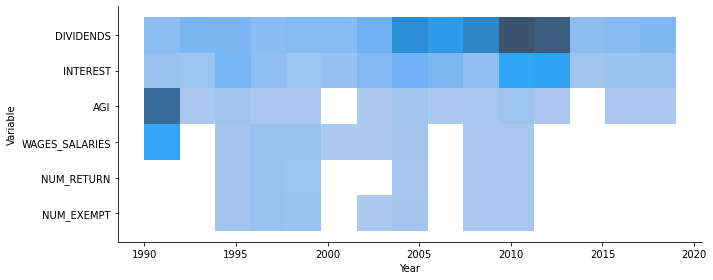
\includegraphics[scale=0.5]{images/data/outlier_distribution.png}}
Note: A darker block indicate a greater number outliers in that block. 
\end{center}

In general, dividend and interest income contain more outliers than the rest of the variables as these sources of income are naturally more sensitive to business cycles and should see larger fluctuations. 

There are two clusters of outliers that are worth noting. The first cluster of outliers fall on AGI and wages and salaries around 1990. This is due to a data error in IRS county data. Data of AGI and wages and salaries appears to be 10 times larger than they should be for Indiana counties in 1989, thus many counties "saw" around 90\% decrease in AGI and wages and salaries. I believe such a uniform and extreme decline is impossible, and therefore is likely an error in the data. IRS Statistics of Income Division has confirmed this issue. 

The second cluster of outliers appear to be dividends and interest income around 2010. This may be a result from the Global Financial Crisis, as we are seeing huge increase in dividend and interest income around 2005-2006, and huge decrease around 2008-2010. The correspondence in timing with boom and bust of the housing, financial, and derivative markets suggests this link. 


\pagebreak

\begin{center}
Figure A.2: Distribution of Outlier Counties by Population\\
\noindent
\makebox[\textwidth]{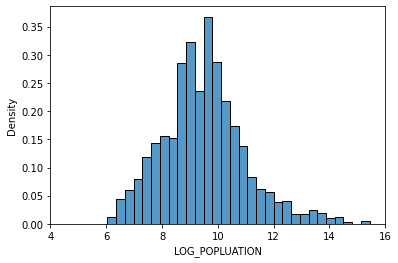
\includegraphics[scale=0.6]{images/data/outlier_pop.png}}
\end{center}

\begin{center}
Figure A.3: Distribution of All Counties by Population\\
\noindent
\makebox[\textwidth]{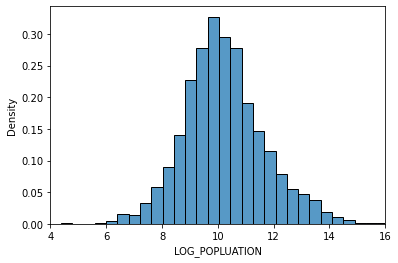
\includegraphics[scale=0.6]{images/data/all_pop.png}}
\end{center}

In addition, I also examine if county size is correlated with the appearance of outliers. The histograms above shows the distribution of population for those counties containing at least one outliers and all counties. It seems the outlier counties are smaller in terms of population. However, the difference is not significant. 

\pagebreak

\subsection*{B. Regression Results with 10\% Cutoff}
\begin{table}[htbp]
\renewcommand\thetable{B.1}
\caption{Dependent Variable: Change in Personal Taxable Income}
\centerline{
    \begin{tabular}{l c c c c}
    \toprule
    \textbf{} & \textbf{(A)} & \textbf{(B)} & \textbf{(C)} & \textbf{(D)}\\ 
    \textbf{Variable} & \textbf{Pooled} & \textbf{Cross-section} & \textbf{Time-series} & \textbf{Two-way fixed} \\
    \midrule
    intercept                          &       3.9118*** &  3.8404***  &       4.2262*** &  4.1468***\\
                                       &      (0.4206)   & (0.0664)    &      (0.0526)   & (0.0538)\\
    change in aggregate income         &       0.1914*** &  0.2322***  &       0.0121    &  0.0574***\\
    {$\times$ high income inequality}  &      (0.0258)   & (0.0170)    &      (0.0128)   & (0.0125)\\
    \midrule
    Time fixed effect                  &       No        &  Yes        &       No        &  Yes        \\
    ZIP code fixed effect              &       No        &  No         &       Yes       &  Yes        \\
    \midrule
    \textbf{$R^2$}                     &       0.0301    &  0.0425     &       8.92e-05    &  0.0018\\
    N. of Observations                 &       11640     &  11640      &       11640     &  11640 \\         
    \bottomrule
    \addlinespace[1ex]
    \multicolumn{3}{l}{\textsuperscript{***}$p<0.01$, 
      \textsuperscript{**}$p<0.05$, 
      \textsuperscript{*}$p<0.1$}
    \end{tabular}
}
\end{table}

\pagebreak
\begin{center}
Figure B.2: Estimated Coefficients for ``Change in Aggregate Income $\times$ High Income Inequality" Using 10-year Subsets for Total Income and Income of Different Sources\\
\noindent
\makebox[\textwidth]{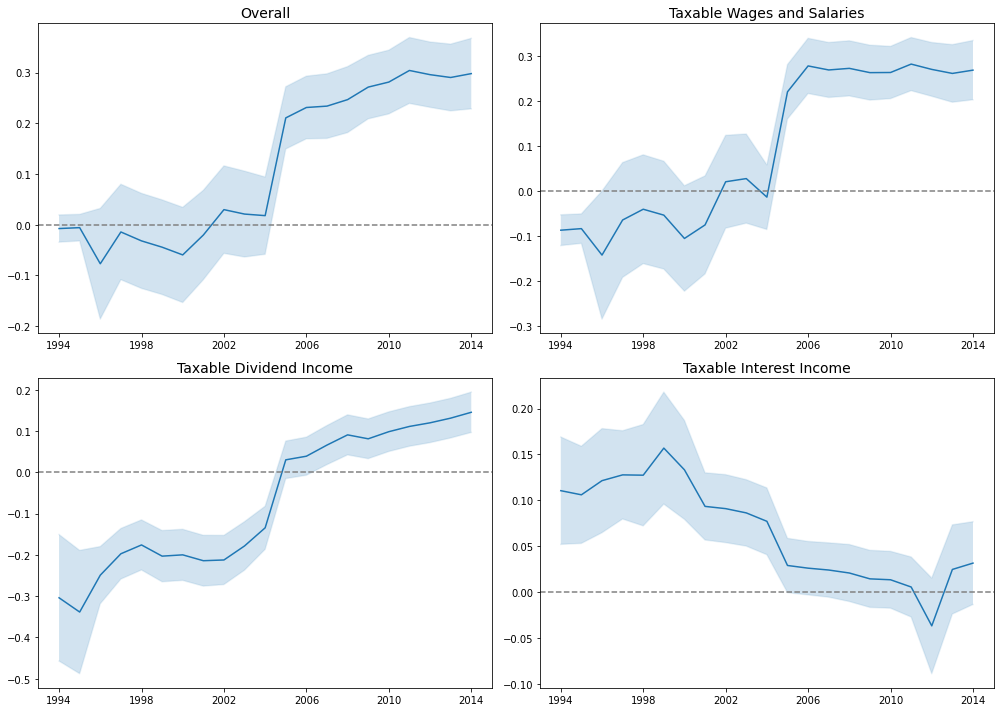
\includegraphics[scale=0.4]{images/robustness/panel_subset_robustness_basic_0.1_0.9.png}}
Note: The estimated coefficients are obtained by performing panel regression with TWFEs on 10-year subsets of county-level data. The horizontal axis specifies the time period for each data subset, where the number represents the "middle"s of 10-year subsets. The bands around the curves are the standard error margins (or 95\% confidence intervals).
\end{center}


\pagebreak

\subsection*{C. Regression Results with 50\% Cutoff}

\begin{table}[htbp]
\renewcommand\thetable{C.1}
\caption{Dependent Variable: Change in Personal Taxable Income}
\centerline{
    \begin{tabular}{l c c c c}
    \toprule
    \textbf{} & \textbf{(A)} & \textbf{(B)} & \textbf{(C)} & \textbf{(D)}\\ 
    \textbf{Variable} & \textbf{Pooled} & \textbf{Cross-section} & \textbf{Time-series} & \textbf{Two-way fixed} \\
    \midrule
    intercept                          &       3.8566*** &  3.8078***  &       4.1859*** &  4.1547***\\
                                       &      (0.0275)   & (0.0286)    &      (0.0231)   & (0.0229)\\
    change in aggregate income         &       0.2055*** &  0.2333***  &       0.0177***    &  0.0355***\\
    {$\times$ high income inequality}  &      (0.0057)   & (0.0068)    &      (0.0051)   & (0.0051)\\
    \midrule
    Time fixed effect                  &       No        &  Yes        &       No        &  Yes        \\
    ZIP code fixed effect              &       No        &  No         &       Yes       &  Yes        \\
    \midrule
    \textbf{$R^2$}                     &       0.0372    &  0.0457     &       0.0002    &  0.0008\\
    N. of Observations                 &       58230     &  58230      &       58230     &  58230 \\         
    \bottomrule
    \addlinespace[1ex]
    \multicolumn{3}{l}{\textsuperscript{***}$p<0.01$, 
      \textsuperscript{**}$p<0.05$, 
      \textsuperscript{*}$p<0.1$}
    \end{tabular}
}
\end{table}

\pagebreak

\begin{center}
Figure C.2: Estimated Coefficients for ``Change in Aggregate Income $\times$ High Income Inequality" Using 10-year Subsets for Total Income and Income of Different Sources\\
\noindent
\makebox[\textwidth]{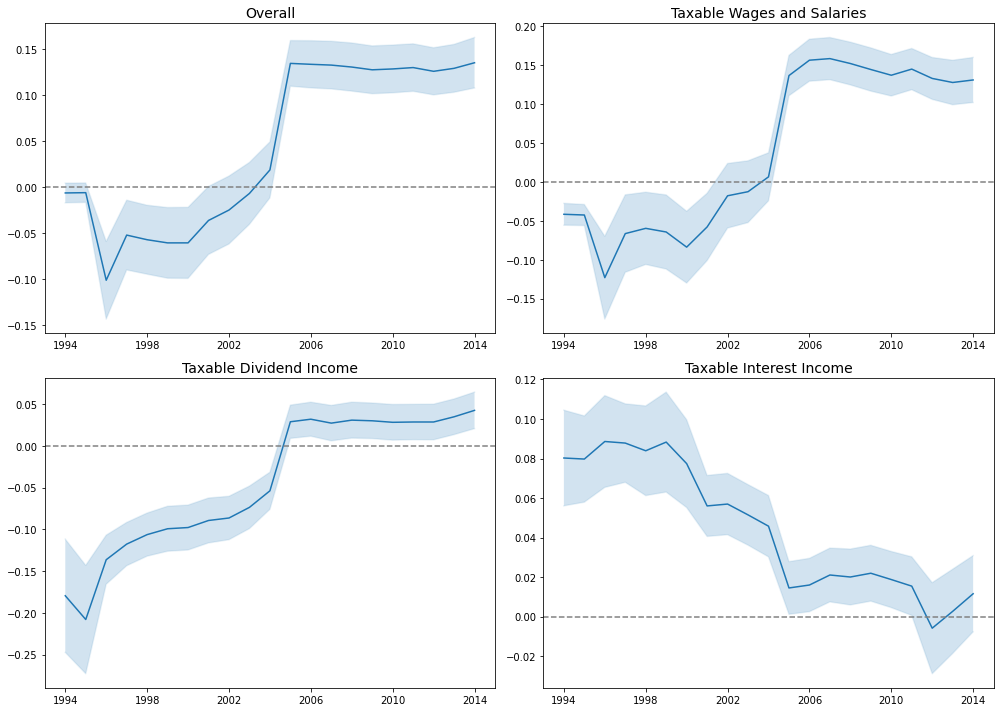
\includegraphics[scale=0.4]{images/robustness/panel_subset_robustness_basic_0.5_0.5.png}}
Note: The estimated coefficients are obtained by performing panel regression with TWFEs on 10-year subsets of county-level data. The horizontal axis specifies the time period for each data subset, where the number represents the "middle"s of 10-year subsets. The bands around the curves are the standard error margins (or 95\% confidence intervals).
\end{center}


\end{document}
